\chapter{Implementation} % (fold)
\label{cha:implementation}

This chapter focuses on software architecture and implementation aspects. We identify key attributes that Legacy must exhibit and describe the adopted approaches to tackle them. Overall, Legacy’s underlying implementation aims at building a robust application that inspires trust for both users and investors.

Legacy’s core functionalities reside in a blockchain platform (more specifically, the Ethereum blockchain). This aspect is perhaps the main competitive advantage of Legacy with respect to similar solutions, and also enables additional functionalities that have not been addressed by other services. Before introducing Legacy’s general architecture, the reasons why a blockchain platform has been adopted are briefly discussed next.


\section{Why Blockchain?} % (fold)
\label{sec:why_blockchain_}

The essential role of a blockchain consists on removing the dependency on trusted third parties in networks where nodes are non-reliable. In this way, any pair of nodes may exchange and process data securely without the intervention of intermediaries. In this way, Bitcoin eliminated the requirement for banks as validators of money transactions. The introduction of smart contracts has paved the way for many novel blockchain applications. Basically, smart contracts not only allow to securely perform peer-to-peer money transactions, but virtually any type of operation. In addition, smart contracts can be executed programmatically and in response to real world events (i.e., events outside of the blockchain). In our context, a blockchain platform supporting smart contracts also allows us to guarantee the main following properties: 

\begin{itemize}
	\item Authenticity: a will stored in the form of a smart contract allows to fully guarantee that all its content was actually dictated by its original author.
	\item Immutability: once a smart contract has been signed and uploaded to the blockchain, it cannot be modified nor deleted by attackers.
	\item Reliability: most blockchains consists of a large number of nodes that jointly validate the current system state. Smart contract data and transaction records are safely stored, validated and replicated at each network node. Hence, It is very difficult for an attacker to disrupt the network or corrupt the data.
\end{itemize}

% section why_blockchain_ (end)

\section{Architecture} % (fold)
\label{sec:architecture}
Legacy’s architecture is composed by several entities: the blockchain platform, Legacy’s own infrastructure, an Oracle---which serves as interface between the smart contracts and the outside world---and other third-party services. In an ideal scenario, third-party services would only be required for providing input data to the PoL engine, whereas most of the application logic would reside in the Blockchain. However, given the current state of maturity of blockchain technologies and related services, some functionalities must be initially implemented using a custom backend as well as third-party infrastructure. As a consequence, Legacy’s architecture is expected to evolve in time, starting from a hybrid architecture and converging towards a fully decentralized architecture.

\subsection{Legacy v1.0 (Memoirs): A Hybrid Architecture} % (fold)
\label{sub:legacy_v1_0_memoirs_a_hybrid_architecture}
Legacy v1.0, named Memoirs, will be the first stable release of the Legacy Project. This initial version enables secure distribution of memories in the form of digital data, such as pictures, videos, text documents, etc. Since blockchain technologies supporting privacy requirements are still evolving, Legacy Memoirs is based on a hybrid architecture, making use of smart contracts but keeping sensitive data on more traditional technologies.
A high-level representation of Legacy Memoirs’ architecture is given in Figure \ref{fig:leg_v1_arch}. Legacy’s own infrastructure and frontends are shown in blue, third-party services in green and the blockchain in red. There are two main frontends: a web application, which is the main interface between the user and the core infrastructure, and a mobile application, which has more limited capabilities and is mainly used for providing PoL data. Legacy’s backend plays different roles. First, it creates smart contract instances after a user initiates the service and commits a capsule. Second, once a user smart contract is uploaded to the blockchain, the backend is in charge of running periodic calls in order to execute the code. And third, it also gathers PoL data from external web services and plugins. The user smart contract implements the PoL algorithm that determines if a user is still alive or not, schedules subsequent calls from the backend and triggers the distribution of capsules once the PoL engine determines that the user has died. 
Memories and capsules will be initially stored using third-party services. Further details are given in Section <storage>.
To allow our smart contracts to query the outside world (for instance, for PoL signalling), an Oracle interface is required. Legacy Memoirs will employ a third-party, Ethereum-compatible Oracle (such us Oraclize).

\begin{figure}[h]
  \centering
  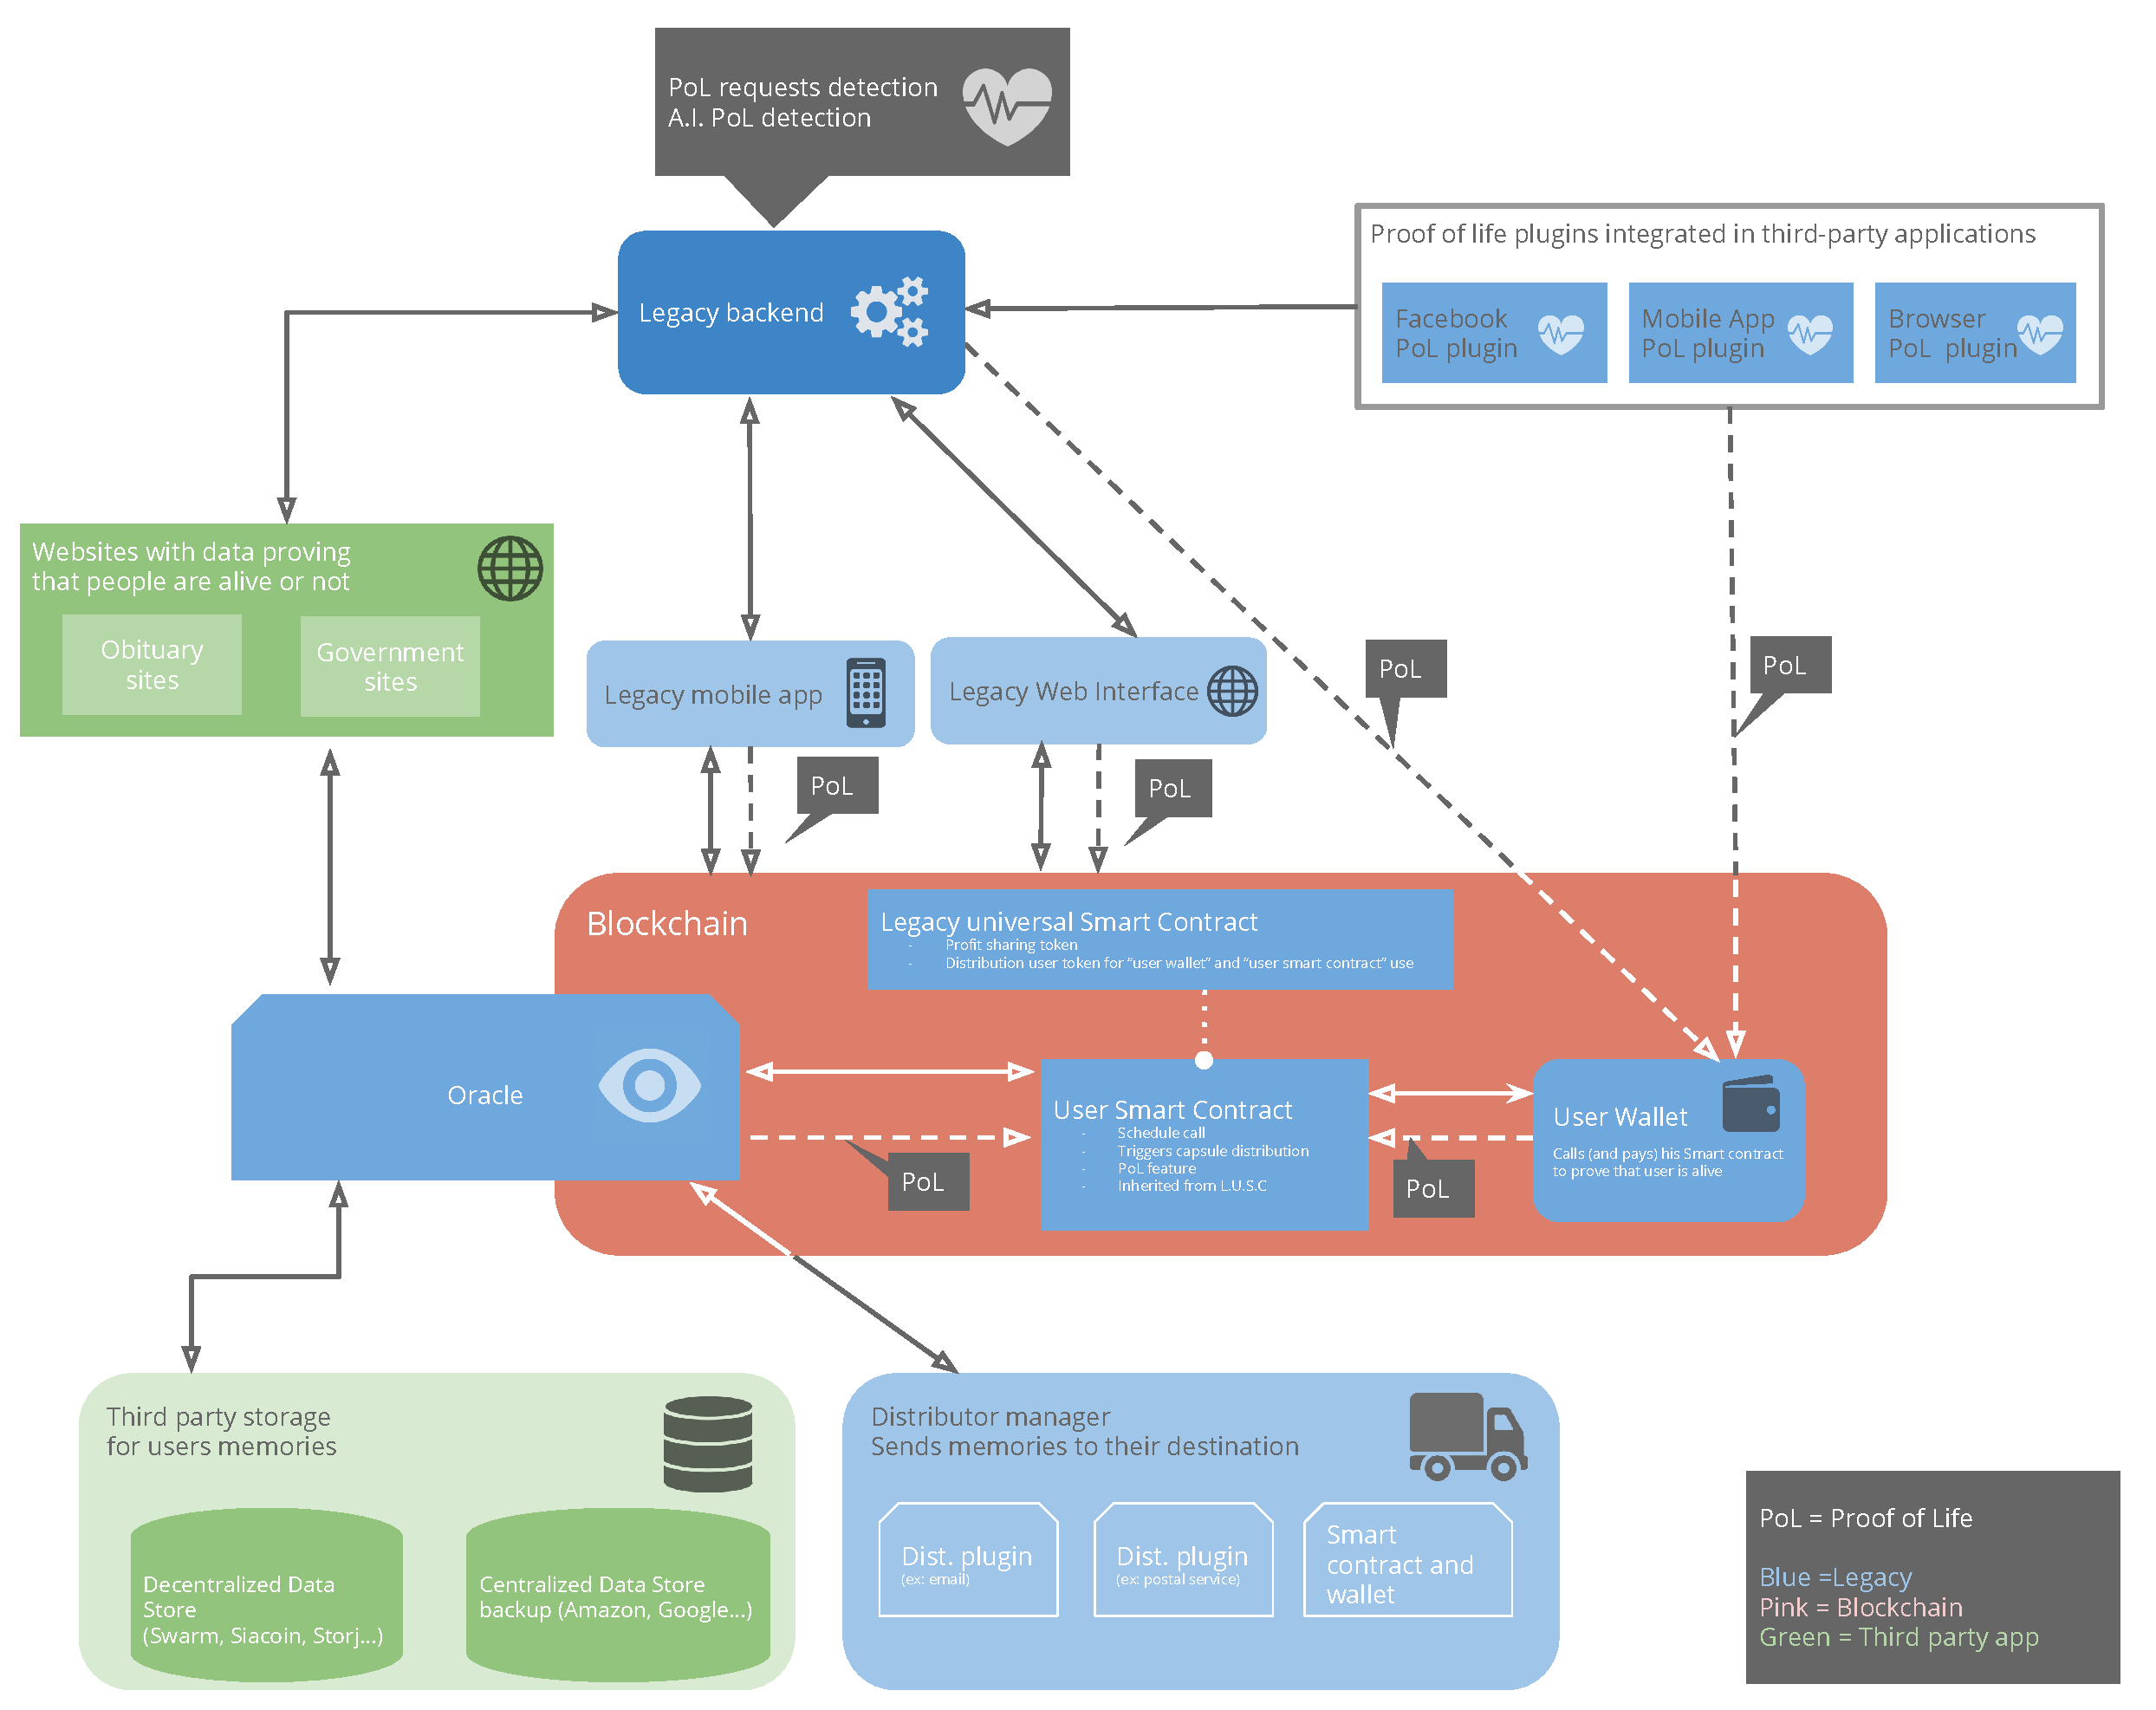
\includegraphics[scale=0.3]{fig/architecture_v02_hybrid}
  \caption{Legacy Mémoires architecture.}
  \label{fig:leg_v1_arch}
\end{figure} 

% subsection legacy_v1_0_memoirs_a_hybrid_architecture (end)

\subsection{Legacy v2.0 (Heritage): Towards a Fully Decentralized Architecture} % (fold)
\label{sub:legacy_v2_0_heritage_towards_a_fully_decentralized_architecture}
Legacy v2.0 Heritage will be Legacy’s second stable release. It main differences with respect to Legacy Memoirs are in the underlying architecture. This version intends to take maximum advantage of blockchain features offering, in particular, on-chain, confidential storage services. Release of this version is estimated for 2020, though it is subject to the technological advances in the blockchain ecosystem.
% subsection legacy_v2_0_heritage_towards_a_fully_decentralized_architecture (end)

% section architecture (end)

\section{Technical Aspects} % (fold)
\label{sec:technical_aspects}

\subsection{Data Storage} % (fold)
\label{sub:data_storage}
Using the Ethereum-based smart contracts guarantees that the code is reliably stored and remains immutable in the long term. However, data storage on the blockchain is currently prohibitively expensive, at more than 1 million USD for 1 Gigabyte. As a consequence, data storage requires another approach for now---though we will continue to closely monitor new services such as Swarm.
Today, reliable data storage means that Legacy will have to maintain multiple copies of the data, on multiple providers around the world.
Currently identified providers are:
Swarm (Decentralized)
Usenet (Decentralized)
Storj (Decentralized)
Sia (Decentralized)
Filecoin (Decentralized)
Local Storage (Centralized)
Glacier by Amazon (Centralized)
hubiC by OVH (Centralized)
Drive by Google (Centralized)

Combining proven and experimental storage methods will allow Legacy to be confident in its longevity promise (see below).

\subsubsection*{Swarm} % (fold)
\label{ssub:swarm}
A blockchain-based file storage is a natural fit for Legacy. Since Swarm is based on the Ethereum blockchain and promises the features we are looking for, we expect Swarm to become our main data store when considered stable and mature (and pricing allows).
Swarm offers the following noteworthy features for Legacy:
\begin{itemize}
	\item Zero downtime
	\item DDOS resistance
	\item Self-sustainability
	\item Fault tolerance
	\item Storage insurance
	\item Data corruption resistance
\end{itemize}
% subsubsection swarm (end)

% subsection data_storage (end)

\subsection{Proof of Life} % (fold)
\label{sub:proof_of_life}

The set of functions by which Legacy determines if a user has died is referred to as Proof of Life (PoL). The PoL engine is implemented at different parts of the application. It is configured by the user through the web interface and, internally, it is commanded by the user smart contract instance. Several different sources of data can be used for PoL purposes, among which we may mention:
Online user activity: simple plugins can be implemented in order to directly signal online user activity. To that end, each user is assigned a personal wallet that serves as interface with the user smart contract. In this way, when a user logs in a given web app, a simple empty transaction can be generated through a web app plugin to the user smart contract. Plugins can be integrated in social networks (e.g. Facebook and Twitter) and on the Legacy web interface as well.
A dedicated mobile app: Legacy may receive direct signalling using a mobile app in which users can simply press a button or answer some personal question.
Email notifications: users can signal activity by clicking on a link sent periodically from Legacy’s servers. 
Official data: Some governments offer official obituary databases that can be freely consulted through an API.  
Human-assisted mechanisms: as an additional PoL layer, Legacy employees may directly contact a person previously designated by the user.

The different PoL signalling channels are shown in Figure \ref{fig:leg_v1_arch}. Using these various input data sources, a weighted algorithm determines the user state (alive/dead) with a given periodicity. The main input parameters, plugins and periodicity are fully configurable by the user, and can be adapted on-the-fly. The options available for PoL also vary according to the user’s subscription package because using additional mechanisms also results in increased transactions between the blockchain and external services, which in turn involves additional costs. 
% subsection proof_of_life (end)

\subsection{Security} % (fold)
\label{sub:security}
[WIP]
The critical parts of our application will reside on the Ethereum blockchain, and will thus be and remain fully auditable by any party. Legacy will have an independent third-party audit major releases. Usage of the web interface will be optional.
% subsection security (end)

\subsection{Privacy} % (fold)
\label{sub:privacy}
On the Legacy contract :
Data (publicly) stored in the smart contract will be anonymized in order to protect our users’ privacy. Only a user will have access to his unique identifiers.

On stored memories :
Files that have profound sentimental values are assigned a higher-than-average level of confidentiality. Protecting the privacy of the Legacy users is thus paramount, and third-party providers cannot be entrusted with this responsibility. All data will be encrypted

On zero-party privacy :
Defining a protocol where only the smart contract, on set conditions, will have access to the data will be a key research focus for Legacy.
% subsection privacy (end)

\subsection{Long-term Service Availability} % (fold)
\label{sub:long_term_service_availability}
Clearly, Legacy must provide guarantees of sustainability in time. In many cases, in fact, user's capsules are transferred within a time span of at least several decades.  Ensuring service operation for such large time spans is one of the most important challenges of Legacy and requires taking multiple measures. 

From the point of view of the application architecture, the code must be able to evolve in time and be easily adaptable according to major technological changes. This is another reason why dependence on specific third-party services must be minimized, in particular on those who are based on centralized architectures. Instead, core functions of Legacy should be flexible and provide support for alternative solutions. In the long term, Legacy expects to be agnostic regarding its main dependencies (i.e. blockchain platform, storage and Oracle interface). This would allow, for instance, to migrate user’s smart contracts from one blockchain to another, in the eventuality that the former shows critical signs of scalability or stability issues. A blockchain-agnostic model also offers the possibility of setting up capsules into two parallel blockchains, if this option appears to be economically viable.    

On the other hand, it is desirable to minimize the dependence on the Legacy organization itself. Indeed, users expect that their capsules will be effectively distributed even in the eventuality that the Legacy organization is dissolved. As mentioned in Section \ref{sec:the_legacy_foundation}, this will be one of the fundamental roles of the Legacy Foundation. Among the measures foreseen in this case, Legacy is committed to publishing an open source application that allows users to keep paying operational costs (i.e., fees required for blockchain transactions and storage) in order to ensure continuous operation. The Legacy foundation will be in charge of maintaining the code and guaranteeing its functionality.
% subsection long_term_service_availability (end)

% section technical_aspects (end)

% chapter implementation (end)